\documentclass[10pt]{beamer}\usepackage[]{graphicx}\usepackage[]{color}
% maxwidth is the original width if it is less than linewidth
% otherwise use linewidth (to make sure the graphics do not exceed the margin)
\makeatletter
\def\maxwidth{ %
  \ifdim\Gin@nat@width>\linewidth
    \linewidth
  \else
    \Gin@nat@width
  \fi
}
\makeatother

\definecolor{fgcolor}{rgb}{0.345, 0.345, 0.345}
\newcommand{\hlnum}[1]{\textcolor[rgb]{0.686,0.059,0.569}{#1}}%
\newcommand{\hlstr}[1]{\textcolor[rgb]{0.192,0.494,0.8}{#1}}%
\newcommand{\hlcom}[1]{\textcolor[rgb]{0.678,0.584,0.686}{\textit{#1}}}%
\newcommand{\hlopt}[1]{\textcolor[rgb]{0,0,0}{#1}}%
\newcommand{\hlstd}[1]{\textcolor[rgb]{0.345,0.345,0.345}{#1}}%
\newcommand{\hlkwa}[1]{\textcolor[rgb]{0.161,0.373,0.58}{\textbf{#1}}}%
\newcommand{\hlkwb}[1]{\textcolor[rgb]{0.69,0.353,0.396}{#1}}%
\newcommand{\hlkwc}[1]{\textcolor[rgb]{0.333,0.667,0.333}{#1}}%
\newcommand{\hlkwd}[1]{\textcolor[rgb]{0.737,0.353,0.396}{\textbf{#1}}}%
\let\hlipl\hlkwb

\usepackage{framed}
\makeatletter
\newenvironment{kframe}{%
 \def\at@end@of@kframe{}%
 \ifinner\ifhmode%
  \def\at@end@of@kframe{\end{minipage}}%
  \begin{minipage}{\columnwidth}%
 \fi\fi%
 \def\FrameCommand##1{\hskip\@totalleftmargin \hskip-\fboxsep
 \colorbox{shadecolor}{##1}\hskip-\fboxsep
     % There is no \\@totalrightmargin, so:
     \hskip-\linewidth \hskip-\@totalleftmargin \hskip\columnwidth}%
 \MakeFramed {\advance\hsize-\width
   \@totalleftmargin\z@ \linewidth\hsize
   \@setminipage}}%
 {\par\unskip\endMakeFramed%
 \at@end@of@kframe}
\makeatother

\definecolor{shadecolor}{rgb}{.97, .97, .97}
\definecolor{messagecolor}{rgb}{0, 0, 0}
\definecolor{warningcolor}{rgb}{1, 0, 1}
\definecolor{errorcolor}{rgb}{1, 0, 0}
\newenvironment{knitrout}{}{} % an empty environment to be redefined in TeX

\usepackage{alltt}%
\setbeamersize{text margin left=0.5cm, text margin right=0.5cm}

\usepackage{alltt}%
\usetheme[background=light]{metropolis} 
\usecolortheme{seahorse}

\usepackage[utf8]{inputenc}%


\usepackage[normalem]{ulem}%strikeout
 

% graphics
%% Figures %%%%%%%%%%%%%%%%%%%%%%%%%%%%%%%%%%%%%%%%%%%%%%%%%%
\usepackage{graphicx}
\usepackage{xcolor}%for color mixing

\usepackage{amsmath}%
\usepackage{amsfonts}%
\usepackage{amssymb}%
\usepackage{graphicx}

\usepackage{tikz}
\usetikzlibrary{calc}

\usepackage{hyperref}

%%%%%%%%%%%%%%%%%%%%%%%%%%%%%%%%%%%%%%%%%%%%%%
%%%%%%%%%%%%%%%%% Doc info %%%%%%%%%%%%%%%%%%%
\title{R-Markdown}
\author{Timoth\'ee Bonnet}
\institute{BDSI / RSB}
\date{\today}

%%%%%%%%%%%%%%%%%%%%%%%%%%%%%%%%%%%%
\IfFileExists{upquote.sty}{\usepackage{upquote}}{}
\begin{document}



\begin{frame}
\centering
\href{https://www.youtube.com/watch?v=s3JldKoA0zw}{
\includegraphics[width=0.8\textwidth]{Figures/markdownyoutube.png}}

\end{frame}
%%%%%%%%%%%

\begin{frame}
\maketitle
\end{frame}
%%%%%%%%%%%

\begin{frame}{What you need:}

\begin{knitrout}\small
\definecolor{shadecolor}{rgb}{0.843, 0.867, 0.922}\color{fgcolor}\begin{kframe}
\begin{alltt}
\hlkwd{install.packages}\hlstd{(}\hlkwd{c}\hlstd{(}\hlstr{"knitr"}\hlstd{,} \hlstr{"xtable"}\hlstd{))}
\end{alltt}
\end{kframe}
\end{knitrout}

\end{frame}
%%%%%%%%%%%

\begin{frame}{Create an R Markdown html document in RStudio}
\centering
\only<1>{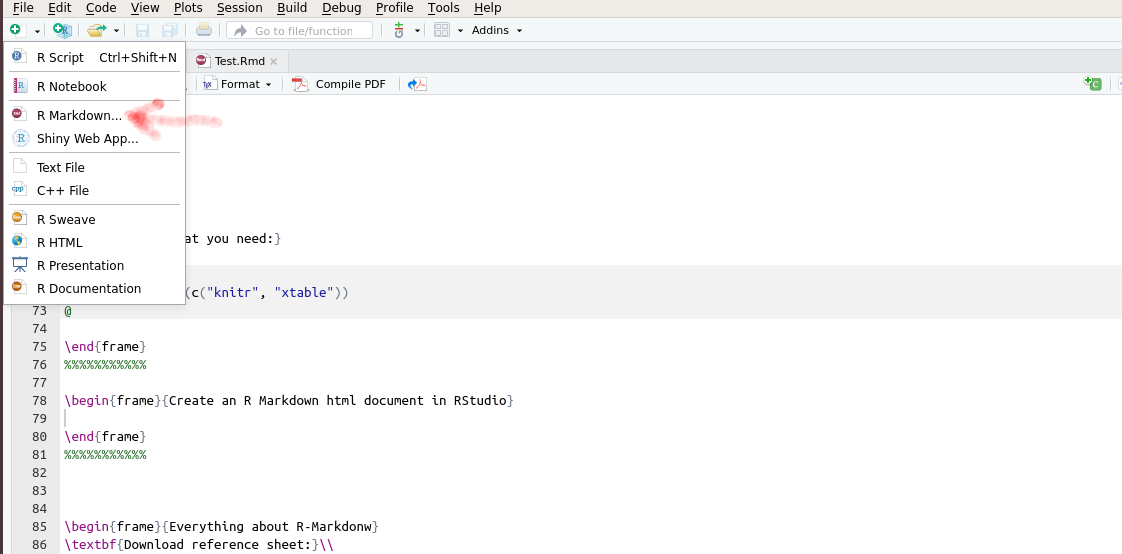
\includegraphics[width=0.8\textwidth]{Figures/Step1.png}}
\only<2>{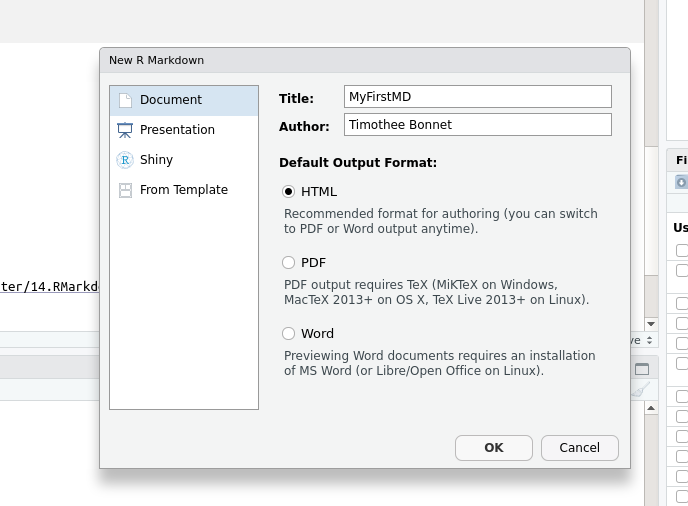
\includegraphics[width=0.8\textwidth]{Figures/Step2.png}}
\only<3>{

\begin{exampleblock}{Components of R-Markdown:}
  \begin{enumerate} 
    \item YAML = Configuration
    \item Text
    \item Code chunks
  \end{enumerate}
\end{exampleblock}

}
\end{frame}
%%%%%%%%%%%

\begin{frame}{Text: Markdown syntax}
  \begin{columns}
    \begin{column}{0.5\textwidth} 
      \uncover<1->{\texttt{Simple text}\\}
      \uncover<2->{\texttt{\# Header (main)} \\}
      \uncover<3->{\texttt{\#\# Header (section)} \\}
      \uncover<4->{\texttt{\#\#\# Header (sub-section)} \\}
    \end{column}
    \begin{column}{0.5\textwidth}
      \uncover<1->{Simple text\\}
      \uncover<2->{\textbf{\LARGE Header (main)} \\}
      \uncover<3->{\textbf{\Large Header (section)} \\}
      \uncover<4->{\textbf{\large Header (sub-section)} \\}
    \end{column}
\end{columns}
\end{frame}
%%%%%%%%%%%%%

\begin{frame}{Everything about R-Markdonw}
\textbf{Download reference sheet:}\\
\url{https://github.com/timotheenivalis/RSB-R-Stats-Biology/raw/master/14.RMarkdown/rmarkdown-reference.pdf}

\textbf{Download quick cheatsheet:}\\
\url{https://github.com/timotheenivalis/RSB-R-Stats-Biology/raw/master/14.RMarkdown/rmarkdown-cheatsheet-2.0.pdf}

\textbf{More resources by RStudio:}\\
\url{https://rmarkdown.rstudio.com/index.html}

\end{frame}
%%%%%%%%%%%
\end{document}
